\documentclass{scrartcl}
%% Alle benodigde pakketjes
%Belangrijke packages voor Schrijven van acenten, trema
\usepackage[utf8]{inputenc}
\usepackage[T1]{fontenc}
\usepackage{helvet}
\usepackage{mathpazo} % Palatino font, een betere font dan standaard. Is serif-font, dus font voor de verhalende tekst
\setkomafont{disposition}{\bfseries\rmfamily}
\addtokomafont{captionlabel}{\bfseries}
%% Eind TypografiePackages


%Taal
\usepackage[dutch]{babel} %Nederlandse Taal
\usepackage{blindtext}
%%

%%%%% Wiskunde Paketjes
\usepackage{amsmath}
\usepackage{amsfonts}
\usepackage{amssymb}
\numberwithin{equation}{section}%Wiskundige formules worden gevolgd door een eerste getal die de behoring van welke sectie aangeeft.
%% Eind WiskundePackages


%%%%% Graphics
\usepackage[table]{xcolor}%%Kleurgeving van columnen, rijen en cellen in tabellen. 
\usepackage{graphicx}%%Externe Foto toevoeger
%\graphicspath{{./Graphics/}}%%Geeft submap van Graphics aan, voor geordend werken.
\usepackage{tikz}%% Intern Graphic Maker
\usetikzlibrary{patterns}
\usetikzlibrary{positioning,calc}
%%

%%%%% Graphs
\usepackage{pgfplots}
\usepackage{pgfplotstable} % Voor linieare trendlijn bij data
\usepackage{filecontents}
%Bij een <\addplot> command moet je bij de optie in <[]> de error bars op het eind van alle opties doen
%%

%SI-eenheden pakket
\usepackage{siunitx}%% Maakt toevoeging van eenheden intuïtiever en als gevolg gemakkelijker
\sisetup{output-decimal-marker = {,}} %De komma wordt gezien als een decimaal-teken bij gebruik van SIunitx pakket. Beter gezegd een punt <.> wordt in het document als een komma afgebeeld, zoals \num{5.59} wordt weergeven als 5,59. ,per-mode=fraction : eenheden die worden gedeeld worden als breuk weergeven.
%%

%%%%%Tabel
\usepackage{array,multirow,booktabs,tabularx}%%Tabellenmaker 1.Array voor horizontale lijn en arraystretch, 2. Multirow en Multicolumn voor merging rijen en columnen respectievelijk, 3.Booktabs voor code commands in tabel. 4. Tabularx voor één table als twee tables naast elkaar op één pagina
\renewcommand{\arraystretch}{1.5}%Ruimte tussen twee rijen
\setlength{\tabcolsep}{10pt}%Ruimte tussen twee colommen 
%\setlength{\heavyrulewidth}{1.1pt}
%%

%Package handig voor Chemische formules en R.V. \ce{H2O}= wordt met subscript geschreven
\usepackage[version=4]{mhchem}
\usepackage{chemfig}
%%

%Handig voor verwijzingen
\usepackage{hyperref}
\usepackage[dutch]{cleveref}
%\crefformat{equation}{vgl.~(#2#1#3)} 
%\Crefformat{equation}{Vgl.~(#2#1#3)} 
%
%\crefformat{table}{tabel.~(#2#1#3)} 
%\Crefformat{table}{Tabel.~(#2#1#3)} 
%%

%Bepaling margegrootte
\KOMAoptions{DIV=calc,BCOR=.75cm, abstract=true}
\usepackage[activate={true,nocompatibility},final,tracking=true,kerning=true,spacing=true,factor=1100,stretch=10,shrink=10]{microtype}
\microtypecontext{spacing=nonfrench}
% activate={true,nocompatibility} - activeert uitsteking van tekst over marge en individuele letters in woorden uit spreiden
% final - zet aan microtype; gebruik "draft" om uit te zetten
% tracking=true, kerning=true, spacing=true - activeert deze technieken
% factor=1100 - voegt 10% toe aan uitsteking hoeveelheid (standaard is 1000)
% stretch=10, shrink=10 - reduceert stretchability/shrinkability (standaard is 20/20)
\usepackage{setspace,typearea}
%%

%%Links gealineerde tabel en figuur bijschriften(caption)
\setcapwidth[l]{\textwidth}
%%

%%Forcering Floats op de plek te blijven waar ze in de code staan met de optie [H].
\usepackage{float}
%%

%Definiëring van subscripts in eenheden in siunitx package
%\DeclareSIQualifier\<naam van de qualifier>{<hier tekst met hoe de qualifier moet worden weergeven>}
%%

%
\begin{document}
%% Titel
%Effe een titel gemaakt met geschikte logo...
\begin{titlepage} 
	\newcommand{\HRule}{\rule{\linewidth}{0.5mm}} % \Hrule is gelijk aan een een horizontale lijn met de lengte van een tekstlijn en dikte van een halve milimeter
	
	\center% Centralisatie van de elementen die volgen na deze command
	
	%------------------------------------------------
	%	Titels/subtitels
	%------------------------------------------------
	
	\textsc{\LARGE Lyceum}\\[1.5cm] % Onze school
	
	\textsc{\Large Kinematica}\\[0.5cm] % Hoofdonderwerp 
	
	\textsc{\large Fysica}\\[0.5cm] % Het vak
	
	%------------------------------------------------
	%	Titel
	%------------------------------------------------
	
	\HRule\\[0.4cm] %\\[<lengte>] is afstand tussen de hoofdtitel en lijn(Hrule)
	
	{\huge\bfseries Valbeweging van de bal}\\[0.4cm] % Hoofdtitel
	
	\HRule\\[1.5cm]
	
	%------------------------------------------------
	%	Schrijvers
	%------------------------------------------------
	
	\begin{minipage}{0.4\textwidth}
		\begin{flushleft} %De tekst begint links
			\large
			\textit{Auteurs}\\
			Fidon \textsc{Namani}\\
			Jorn \textsc{Smit} % Ik 
		\end{flushleft}
	\end{minipage}
	 % Dit golfje geeft aan dat deze twee minipagina's nooit onder elkaar mogen komen te staan.
	\begin{minipage}{0.4\textwidth}
		\begin{flushright} %De tekst begint rechts
			\large
			\textit{Beoordeler}\\
			D.\textsc{Hamburger} % Jij
		\end{flushright}
	\end{minipage}


	
	%------------------------------------------------
	%	Datum
	%------------------------------------------------
	
	\vfill\vfill\vfill % De datumverschijning is 3/4 lengte van top van papier geplaatst.
	
	{\large\today} % Datum
	
	%------------------------------------------------
	%	Logo
	%------------------------------------------------
	
	\vfill\vfill
	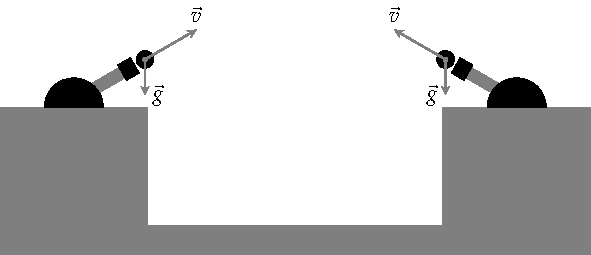
\includegraphics[width=0.75\textwidth]{Cannon.pdf}\\[1cm] % Ons fysica logootje
	 
	
	\vfill %De datum wordt voor de zekerheid nog 1/4 deel van de bodem van papier naar boven geduwd
\end{titlepage}
%%

%
\tableofcontents
\newpage
\section*{Inleiding}\label{sec:Inleiding}
\addcontentsline{toc}{section}{\nameref{sec:Inleiding}}
In de Middeleeuwen waren kastelen essentieel voor de beheersing van de landbouwgrond. Het behouden van de kastelen was dus van heel groot belang. Daarom bezaten kastelen allerlei verdedingswerktuigen. E\'{e}n van deze werktuigen is hete kokend olie. De hete kokende olie werd vanaf de muren van het kasteel op de belegers naar beneden gegooid. Hoeveel tijd zouden de belegers hebben om te ontsnappen van de olie? Beantwoording vereist een analyse van de valbeweging van de olie. Deze analyse is ook afleidbaar door de valbeweging van een ander object te onderzoeken.
\par
In deze proef werd de valbeweging van een bal geanalyseerd met behulp van een videometing en \textit{Coach7}. De beantwoording van de volgende vragen was beoogd:
\begin{description}
\item[Hoofdvraag] Wat voor type beweging is de valbeweging van de bal?
\begin{description}
\item[Deelvraag 1] Wat is het verband tussen de verplaatsing van de bal en de tijd?
\item[Deelvraag 2] Wat is het verband tussen de snelheid van de bal en de tijd?
\end{description}
\end{description}
%
\section{Theorie}
Op aarde is de gravitatieversnelling $g=\SI{9.81}{\meter\per\second}$. Een object die in een rechte beweging naar beneden valt, ondervindt ook luchtweerstand ($\vec{F_{l}}$). Volgens de 2\textsuperscript{de} wet van Newton is de netto kracht op een vallende object gelijk aan \cref{eq:Newton}:
%% Newton equation
\begin{equation}\label{eq:Newton}
\vec{F}_{\mathrm{netto}}=\vec{F}_{z}+\vec{F}_{l} \rightarrow
m\vec{a}=m\vec{g}+\vec{F}_{l}\mathrm{.}
\end{equation}
%%
Als $\vec{F}_{l} \approx \SI{0}{\newton}$ dan geldt voor $\vec{a}$ bij benadering:
%%
\begin{equation*}
\vec{a}\approx \vec{g}\mathrm{.}
\end{equation*}
%%
In \cref{eq:1Integratie} wordt $a$ geïntegreerd naar de tijd ($t$) gemeten in secondes (\si{\second}).\footnote{Integreren is de inverse van differenteren, zoals delen de inverse is van vermenigvuldigen.} Deze integratie levert een vergelijking op van de snelheid $(v)$ in \si{\meter\per\second} als functie van $t$. Deze vergelijking beschrijft een liniear verband tussen $v$ en $t$.
%% Eerste integratie
\begin{equation}\label{eq:1Integratie}
v(t)=\int g dt= gt + v_i
\end{equation}
%%
Wanneer \cref{eq:1Integratie} ge\"{i}ntegreerd wordt, wordt \eqref{eq:2Integratie} verkregen:
%% Tweede integratie
\begin{equation}\label{eq:2Integratie}
y(t)=\int (gt + v_i)dt =\frac{1}{2}gt^2+v_{i}t+y_i\mathrm{.}
\end{equation}
%%
\Cref{eq:2Integratie} beschrijft een functie tussen de eindhoogte $(y)$ in meter (\si{\meter}) en $t$. In de proef begint de valbeweging van de bal in rust. \Cref{eq:2Integratie} kan dus herleid worden tot:
%%
\begin{equation*}
y(t)=\frac{1}{2}gt^2+y_i\mathrm{.}
\end{equation*}
%%
Op basis van de bovengenoemde theorie waren de volgende hypotheses opgesteld, indien $\vec{F_{l}} \approx \SI{0}{\newton}$ gedurend de val:
\begin{itemize}
 \renewcommand{\labelitemi}{\scriptsize$\blacksquare$}
\item De valbeweging is een eenparige versnelde beweging.
\item Een kwadratische verband bestaat tussen $y$ en $t$.
\item Een liniear verband bestaat tussen $v$ en $t$.
\end{itemize}
%
\section{Methode}
E\'{e}n individu hield een lichte voetbal vast op een hoogte $(y_i)$ van \SI{1.80}{\meter} in een windstille ruimte (\cref{fig:Valbeweging}). Deze hoogte werd gemeten met een meetlint met een \SI{+-1}{\centi\meter} precisie. Een andere individu nam de valbeweging op met een moderne smartphone. In verband met overschakeltijd van fotografie- naar opname-mode was de opname gestart voor de val. Dit deel van de opname en de stuiterbeweging aan het eind van de opname waren verwijderd met behulp van \textit{Windows Movie Maker}. De resulterende opname werd ingevoerd in \textit{Coach7}. Met behulp van de videometingcapaciteiten van \textit{Coach7} was $y$ en $v$ bepaald op \num{17} verschillende tijdstippen. De tijdsinterval was constant gehouden bij de \num{17} verschillende tijdstippen.
%% Methode Tikzpicture
\begin{figure}[t]
\centering
\resizebox{.75\textwidth}{!}{%
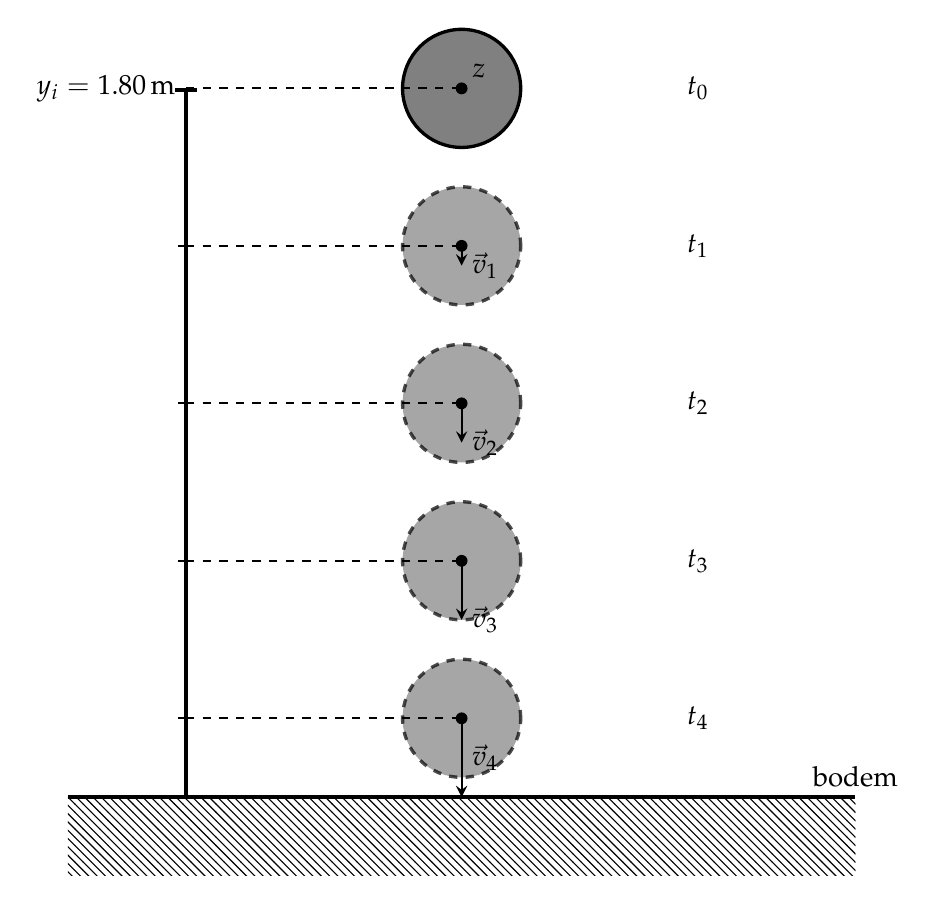
\begin{tikzpicture}[grid/.style={very thin,gray}, xstep=.5cm, ystep=.5cm]
%\draw[grid] (0,0) grid (10,10);
%	\foreach \x in {0,0.5,...,10}
%	\node[anchor=north] at (\x,0) {\x};
%	\foreach \y in {0,0.5,...,10}
%	\node[anchor=east] at (0,\y) {\y};	
\fill[pattern=north west lines] (0,0) rectangle (10,1) node[anchor=south] {bodem};
\draw[ultra thick] (0,1) -- (10,1);
\filldraw[fill=gray, very thick] (5,10) circle[radius=.75cm] node[anchor=south west] {$z$};
\fill (5,10) circle[radius=.075cm];
\draw[very thick,-|] (1.5,1) --(1.5,10) node[anchor=east] {$y_i=\SI{1.80}{\meter}$};
\foreach \y in {2,4,6,8}
\draw[thick] (1.4cm,\y) -- (1.6,\y);
\foreach \y in {2,4,6,8}
\filldraw[fill=gray, very thick, dashed, opacity=0.7] (5,\y) circle[radius=.75cm]; 
\foreach \y in {2,4,6,8}
\fill (5,\y) circle[radius=.075cm];
\draw[->,>=stealth,thick] (5,8) -- (5,7.75) node[anchor= west] {$\vec{v}_1$};
\draw[->,>=stealth,thick] (5,6) -- (5,5.5) node[anchor=west] {$\vec{v}_2$};
\draw[->,>=stealth,thick] (5,4) -- (5,3.25) node[anchor= west] {$\vec{v}_3$};
\draw[->,>=stealth,thick] (5,2) --  node[anchor=west] {$\vec{v}_4$} (5,1);
\node at (8,10) {$t_0$};
\node at (8,8) {$t_1$};
\node at (8,6) {$t_2$};
\node at (8,4) {$t_3$};
\node at (8,2) {$t_4$};
\foreach \y in {2,4,6,8,10}
\draw[thick,dashed] (1.5,\y)-- (5,\y);
\end{tikzpicture}
}
\caption{Een schematische weergave van metingsprincipe. Op een beginhoogte $y_i=\SI{1,80}{\meter}$ werd op gelijke tijdsintervallen de eindhoogte $y_f$ en $v$ bepaald.}
\label{fig:Valbeweging}
\end{figure}

%
\newpage
\section{Resultaten \& Discussie}
\subsection{Resultaten}
Bij de uitvoering van de beschreven methode was de data in \cref{tab:Kwadraat} verkregen. De data vertoonde een kwadratisch verband tussen $y$ en $t$.  Deze vondst was in overeenkomtst met de hypotheses.
De kwadratische verband tussen $y_f$ en $t$ wordt bevestigd en gevisualiseerd in \cref{fig:kwadraat}.
\begin{figure}\label{fig:kwadraat}
\centering
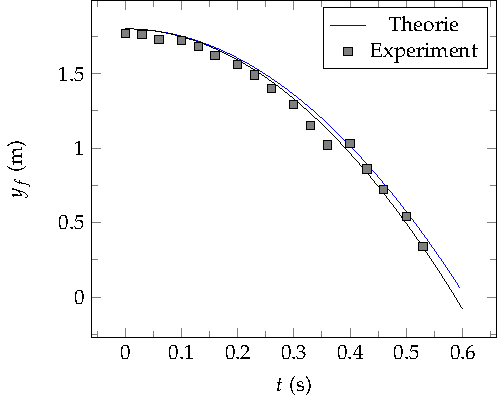
\includegraphics[scale=1]{Grafiekvalbeweging.pdf}
\captionbelowof{figure}{De grafiek met $y_f$ uitgezet tegen $t$ van het experiment en de theorie. Een kwadratische verband bestaat tussen de de verplaatsing en tijd.}
\end{figure}
Verder was gebleken dat een linieare verband bestaat tussen $v$ en $t$. De linieare verband is weergeven in \cref{fig:liniear}. De richtingsco\"{e}ffici\"{e}nt, oftewel $\vec{a}$, wordt weergeven in \cref{eq:Acceleratie}:
%%
\begin{equation}\label{eq:Acceleratie}
\vec{a}=\frac{\Delta \vec{v}}{\Delta t}=\frac{\SI{0}{\meter\per\second}-\SI{-6}{\meter\per\second}}{\SI{0}{\second}-\SI{0.6}{\second}}=\SI{-10}{\meter\per\second\squared}\mathrm{.}
\end{equation}
%%
\begin{figure}[t]
\centering
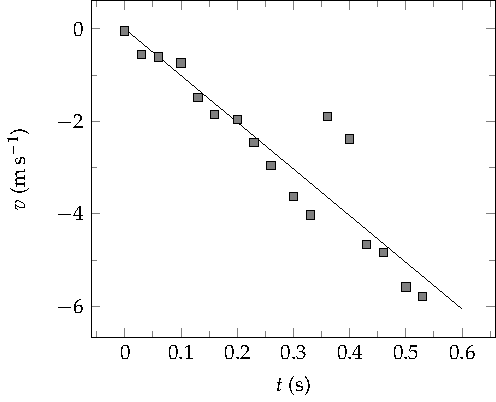
\includegraphics[scale=1]{v,t-grafiek.pdf}
\captionbelowof{figure}{De grafiek met $v$ als functie van $t$. Een liniear verband bestaat tussen $v$ en $t$. De twee meetfouten wijken duidelijk af van de overige datapunten.}
\label{fig:liniear}
\end{figure}
%%
\subsection{Discussie}
De gestelde hypotheses waren positief. De valbeweging was een eenparige versnelde beweging. Een kwadratische verband bestond tussen $y_f$ en $t$. Verder leverde de grafiek met $v$ uitgezet tegen $t$ een rechte op. De valbeweging van de lichte voetbal week echter af van de realiteit. De gevonden waarde voor $a$ was groter dan $g$. De percentuele fout tussen de gevonden en realistische waarde is weergeven in \cref{eq:RelatieveFout}:
%%
\begin{equation}\label{eq:RelatieveFout}
\delta \, g=\frac{a-g}{g}\times 100= \frac{\SI{10}{\meter\per\second\squared}-\SI{9.81}{\meter\per\second\squared}}{\SI{9.81}{\meter\per\second\squared}}=\SI{1.9}{\percent}\mathrm{.}
\end{equation}
%%
Een hogere $g$ zou betekenen dat een object sneller valt onder dezelfde omstandigheden in de ruimte waar de proef is afgenomen dan elders op de wereld. In \cref{fig:kwadraat} neemt $\frac{d^2y_f}{dt^2}$ toe bij latere tijdstippen. Dit is te verwijten aan het gebrek van stroboscopische capaciteit op de smartphone. Hierdoor was het beeld van de bewegende bal wazig op latere tijdstippen. Dit resulteerde in onnauwkeurigheid in de positie van het zwaartepunt van de bal. Als gevolg werd het zwaartepunt repeterend te laag gekozen op latere tijdstippen in \textit{Coach7}. Deze systematische fouten leiden tot een hogere $\frac{d^2y_f}{dt^2}$ en dus hogere $g$.
%
\section{Conclusie}
Concluderend was de valbeweging van de bal geanalyseerd met een smartphone en de videometingcapaciteiten van \textit{Coach7}. De valbeweging was eenparig versneld met een kwadratisch verband tussen $y_f$ en $t$ en een liniear verband tussen $v$ en $t$.
\section{Reflectie}
We zijn tevreden met de resultaten van ons uitgevoerde onderzoek. Daarnaast zijn we trots op ons verslag. De gegevens zijn op een professionele manier in het verslag verwerkt met een mooie strakke lay-out. We zijn minder tevreden met de meetfouten die zijn gemaakt. Ondanks dat we theorie goed hebben toegepast. We hebben in deze PO geleerd om onze kennis in een praktische opdracht toe te passen, waardoor we de onderzoekverslagen hebben kunnen beantwoorden.
\newpage
\appendix
\section{Tabellen}
\begin{center}
\captionaboveof{table}{De \num{17} verschillende tijdstippen met daarbij horende hoogte en snelheid. De 13\textsuperscript{de} en 14\textsuperscript{de} meting, de grijs gekleurde cellen, bevatten een meetfout.}
\begin{tabular}{*{4}{S[table-format=1.2]}}
\toprule
{Meting} & {$t$ (\si{\second})} & {$y_f$ (\si{\meter})} & {$v$ (\si{\meter\per\second})}\\
\midrule
1& 0	 & 1.77&-0.05 \\
2& 0.03 & 1.76&-0.56 \\
3 &0.06 & 1.73&-0.61 \\
4 &0.10 & 1.72&-0.74 \\
5 &0.13 & 1.68&-1.48 \\
6 &0.16 & 1.62&-1.85 \\
7 &0.20 & 1.56&-1.96 \\
8 &0.23 & 1.49&-2.46 \\
9 &0.26 & 1.40&-2.96 \\
10 &0.30 & 1.29&-3.62 \\
11 &0.33 & 1.15&-4.02 \\
12 &0.36 & 1.02&\cellcolor{gray}-1.90 \\
13 &0.40 & \cellcolor{gray}1.03&\cellcolor{gray}-2.38 \\
14 &0.43 & 0.86&-4.66 \\
15& 0.46 & 0.72&-4.84 \\
16 &0.50 & 0.54&-5.58 \\
17& 0.53 & 0.34&-5.79 \\
\bottomrule
\end{tabular}
\label{tab:Kwadraat}
\end{center}
%
\newpage
\section{Logboek}
%\rowcolors{2}{gray!10!}{}
\begin{center}
  \captionaboveof{table}{Een logboek met de activiteit, week van uitvoering, tijdspendering en de uitvoerder.}
\begin{tabular}[center]{*4c}
\toprule
Week van uitvoering & Tijd (\si{\hour})& Activiteit & Uitvoerder\\
\midrule
47 & n.v.t. & n.v.t. & n.v.t.\\
48 &n.v.t.  & n.v.t. & n.v.t.\\
49 & n.v.t. &ori\"{e}ntatie& F/J\\
50 &  n.v.t.&  ori\"{e}ntatie&F/j \\
51 &  2     &videometing  &Fidon \\
52 &  $3\frac{1}{2}$     &dataverwerking  &Fidon \\
1  &  $3\frac{1}{2} $    &afronding  &Jorn \\
2 &  $\frac{1}{6}$&printen  &Fidon \\
\bottomrule
\end{tabular}
\end{center}
\end{document}
